\documentclass{article}
\usepackage{graphicx}
\usepackage{listings}
\usepackage{xcolor}
\usepackage{hyperref}
\usepackage{url}
\title{Decoding Emotions: The Facemood Library for Facial Expression Analysis}
\author{Emir Kaan Özdemir}
\date{August 2024}

\lstdefinestyle{customPython}{
    language=Python,
    backgroundcolor=\color{lightgray},
    basicstyle=\ttfamily\footnotesize,
    keywordstyle=\color{blue},
    commentstyle=\color{green},
    stringstyle=\color{red},
    numbers=left,
    numberstyle=\tiny\color{gray},
    stepnumber=1,
    numbersep=5pt,
    tabsize=4,
    breaklines=true,
    captionpos=b
}

\begin{document}


\maketitle

\begin{abstract}
Facial expression recognition has become an essential tool in both psychological research and practical applications, providing information on human emotions and social interactions. The facemood library is designed to bridge the gap between AI-driven emotion detection and psychological analysis, offering a robust framework for interpreting facial cues. Using advanced machine learning techniques, facemood not only detects basic emotions but also identifies subtle nuances in expression, enabling a deeper understanding of emotional states. This tool is particularly valuable in psychological studies, where accurate emotion detection can enhance the reliability of research findings. Moreover, facemood's potential applications extend to areas such as human-computer interaction, mental health monitoring, and adaptive user interfaces, underscoring its relevance in both academic and practical domains. 
\end{abstract}

\vspace{7cm}

\tableofcontents

\vspace{4cm}

\section{Introduction}
Facial expression recognition plays a crucial role in various fields, including psychological research and human-computer interaction. Understanding and interpreting human emotions through facial expressions provides valuable insights into emotional states and social interactions. This paper introduces the facemood library, a comprehensive tool designed to facilitate emotion recognition from facial expressions using advanced machine learning techniques. In this article, the structure of the multi-classification model and the general CNN model are discussed separately. However, some of the mathematical representations are separate and difficult to understand. In this article, artificial intelligence help is taken [1].

\vspace{0.5cm}

The facemood library bridges the gap between artificial intelligence-driven emotion detection and psychological analysis by offering an intuitive and effective solution for interpreting facial cues. The library is built upon sophisticated algorithms that analyze facial expressions and classify them into different emotional categories. It provides users with both pre-trained models and tools to train custom models, making it adaptable to various applications.

\vspace{0.5cm}

In practical terms, facemood can be used for a wide range of purposes, such as enhancing user experiences in interactive applications, monitoring mental health, and conducting psychological studies. Its capabilities include real-time emotion detection from video feeds, classification of emotional states, and the ability to tailor models to specific datasets.

\vspace{0.5cm}

The development of facemood integrates research from computer science, psychology, and affective computing, resulting in a tool that is not only academically sound but also highly applicable in real-world scenarios. Using the facood library, users can gain a deeper understanding of emotional expressions, contributing to advancements in both theoretical and practical domains of emotion recognition.

\vspace{7cm}

\section{Theoretical and Mathematical Explanations}

\subsection{Model's Explanation}

`facemood` uses a machine learning model to detect the emotion. This model is a CNN (Convolutional Neural Network) model widely used to classify images.

\begin{figure}[h]
    \centering 
    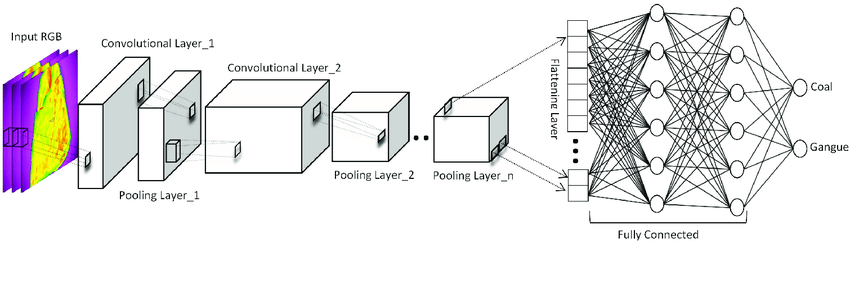
\includegraphics[width=10cm,height=5cm]{image1.png}
    \caption{CNN model working logic. Representation.[2]}
    \label{fig:w_logic}
\end{figure}

\vspace{3cm}

\subsection{Key Components of CNN}

\subsubsection{Convolutional Layer}
\textbf{Description:} This layer applies small filters to input data to create feature maps. Filters learn different features from various parts of the image. \\
\textbf{Function:} Extracts specific features from the image, such as edges, corners, and textures. \\
\textbf{Mathematical Representation:} 
The convolution operation can be represented as:
\begin{equation}
    X_{i,j} = \sum_{m,n} K_{m,n} \cdot I_{i+m,j+n} + b
\end{equation}
where \( X_{i,j} \) is the output value at position \( (i, j) \), \( K \) is the filter (kernel), \( I \) is the input image, and \( b \) is the bias term.

\subsubsection{Activation Function}
\textbf{Description:} Activation functions like ReLU (Rectified Linear Unit) are used. They enable the model to learn non-linear relationships. \\
\textbf{Function:} Helps the model learn non-linear features. \\
\textbf{Mathematical Representation:}
The ReLU activation function is defined as:
\begin{equation}
    f(x) = \max(0, x)
\end{equation}
where \( x \) is the input to the function, and \( f(x) \) is the output after applying the ReLU.

\subsubsection{Pooling Layer}
\textbf{Description:} This layer summarizes and reduces the size of feature maps obtained from the convolutional layer. \\
\textbf{Function:} Reduces the dimensionality of feature maps and the computational cost. \\
\textbf{Mathematical Representation:}
For max pooling, the output is the maximum value within the pooling window:
\begin{equation}
    P_{i,j} = \max_{m,n} \{ F_{i+m,j+n} \}
\end{equation}
where \( P_{i,j} \) is the pooled value, and \( F \) is the feature map from which the maximum is taken within the pooling window.

\subsubsection{Fully Connected Layer}
\textbf{Description:} This layer connects all neurons from the previous layers to every neuron in this layer. \\
\textbf{Function:} Transforms the features into high-level representations for classification or regression tasks. \\
\textbf{Mathematical Representation:}
The output of a fully connected layer is computed as:
\begin{equation}
    y = \sigma(Wx + b)
\end{equation}
where \( W \) is the weight matrix, \( x \) is the input vector, \( b \) is the bias, and \( \sigma \) is the activation function applied to the output.

\subsubsection{Normalization Layer}
\textbf{Description:} Techniques like Batch Normalization normalize the distribution of features. \\
\textbf{Function:} Accelerates training and improves the stability of the model. \\
\textbf{Mathematical Representation:}
Batch Normalization can be represented as:
\begin{equation}
    \hat{x} = \frac{x - \mu}{\sqrt{\sigma^2 + \epsilon}}
\end{equation}
where \( \mu \) and \( \sigma^2 \) are the mean and variance of the batch, \( \epsilon \) is a small constant to avoid division by zero, and \( \hat{x} \) is the normalized output.

\subsection{How CNNs Work}

\begin{enumerate}
    \item \textbf{Input Data:} Typically starts with an image.
    \item \textbf{Convolution Operation:} Filters are applied to generate various feature maps.
    \item \textbf{Activation and Pooling:} Features are processed using activation functions and pooling layers, reducing dimensions.
    \item \textbf{Fully Connected Layers:} Features are flattened and passed through fully connected layers for final classification or regression tasks.
    \item \textbf{Output:} Provides results such as classification or regression outcomes based on the final layer.
\end{enumerate}

\vspace{5cm}

\section{7-Class Classification CNN Model}

The facemood library employs a Convolutional Neural Network (CNN) model for 7-class classification tasks. This section provides a detailed explanation of the model components and their mathematical representations.

\subsection{Overview}
The CNN model used in facemood is designed to classify facial expressions into one of seven distinct emotional categories. The architecture typically includes multiple convolutional layers, activation functions, pooling layers, fully connected layers, and an output layer with softmax activation.

\subsection{Model Architecture}

\subsubsection{Convolutional Layers}
\textbf{Description:} Convolutional layers apply multiple filters to the input image to extract hierarchical features such as edges, textures, and shapes. \\
\textbf{Mathematical Representation:} 
Each convolutional operation can be represented as:
\begin{equation}
    X_{i,j} = \sum_{m,n} K_{m,n} \cdot I_{i+m,j+n} + b
\end{equation}
where \( X_{i,j} \) is the output feature map value, \( K \) is the convolutional kernel, \( I \) is the input image, and \( b \) is the bias.

\subsubsection{Activation Functions}
\textbf{Description:} Activation functions introduce non-linearity into the model, allowing it to learn complex patterns. ReLU is commonly used. \\
\textbf{Mathematical Representation:}
For the ReLU function:
\begin{equation}
    f(x) = \max(0, x)
\end{equation}

\subsubsection{Pooling Layers}
\textbf{Description:} Pooling layers reduce the spatial dimensions of feature maps, retaining important information while lowering computational cost. \\
\textbf{Mathematical Representation:}
For max pooling, the operation is:
\begin{equation}
    P_{i,j} = \max_{m,n} \{ F_{i+m,j+n} \}
\end{equation}
where \( P_{i,j} \) is the pooled value, and \( F \) is the feature map.

\subsubsection{Fully Connected Layers}
\textbf{Description:} Fully connected layers integrate features from previous layers to produce class scores. \\
\textbf{Mathematical Representation:}
The output from a fully connected layer is computed as:
\begin{equation}
    y = \sigma(Wx + b)
\end{equation}
where \( W \) is the weight matrix, \( x \) is the input vector, \( b \) is the bias, and \( \sigma \) is the activation function (e.g., ReLU).

\subsubsection{Output Layer}
\textbf{Description:} The output layer uses a softmax function to convert the raw scores into probabilities for each class. \\
\textbf{Mathematical Representation:}
The softmax function is defined as:
\begin{equation}
    p_i = \frac{e^{z_i}}{\sum_{j} e^{z_j}}
\end{equation}
where \( p_i \) is the probability of class \( i \), and \( z_i \) is the raw score (logit) for class \( i \).

\subsection{Training and Loss Function}
\textbf{Loss Function:} For multi-class classification, the categorical cross-entropy loss is commonly used. \\
\textbf{Mathematical Representation:}
\begin{equation}
    L = -\sum_{i} y_i \log(p_i)
\end{equation}
where \( y_i \) is the true label (one-hot encoded) and \( p_i \) is the predicted probability.

\subsection{Summary}
The CNN model used in facemood processes input images through multiple convolutional and pooling layers to extract features, applies activation functions to introduce nonlinearity, and uses fully connected layers to integrate features for classification. The output layer applies softmax to produce class probabilities, and the model is trained using categorical cross-entropy loss.

\vspace{3cm}

\section{How to Use?}
\subsection{Installation}
To install facemood, you can use pip. You can either install it from PyPI or directly from the source.
\begin{lstlisting}[style=customPython]
pip install facemood
\end{lstlisting}
\subsection{Usage}
\begin{lstlisting}[style=customPython]
from facemood import EmotionRecognizer
emotion_predictor.predict_emotion_from_camera()
\end{lstlisting}

\vspace{1cm}

The function performs real-time emotion recognition using a webcam. Here's a summary of its functionality:

\begin{enumerate}
    \item \textbf{Image Processing:} Captures frames from the webcam, processes them by resizing and normalizing, and prepares them for the model.
    \item \textbf{Emotion Prediction:} Uses a pre-trained machine learning model to predict the emotion based on facial expressions in the images.
    \item \textbf{Display Results:} Overlays the predicted emotion on the video feed and displays it on the screen.
    \item \textbf{Exit Mechanism:} Continues processing until the user presses 'Enter', after which it stops the video feed and closes the window.
\end{enumerate}
\subsection{Requirements(Used Libraries)}
\begin{enumerate}
    \item \textbf{OpenCV:} OpenCV[3] (Open Source Computer Vision Library) is a library of programming functions mainly for real-time computer vision.
    \item \textbf{Pillow:} Python[4] Imaging Library is a free and open source library for the Python programming language that adds support for opening, manipulating, and saving many different image file formats.
    \item \textbf{NumPy:} NumPy[5] is a library for the Python programming language, adding support for large, multi-dimensional arrays and matrices, along with a large collection of high-level mathematical functions to operate on these arrays.
    \item \textbf{TensorFlow:} TensorFlow[6] is a free and open source software library for machine learning and artificial intelligence. It can be used across a range of tasks but has a particular focus on training and inference of deep neural networks.
\end{enumerate}

\vspace{4cm}

\section{Some General Information}
\subsection{Source Code}
You can find the source code here: https://github.com/emirkaanozdemr/facemood
\subsection{PYPI Link}
PYPI Link:
https://pypi.org/project/facemood/1.0.1/

\vspace{7cm}

\section{References and Citations}
\begin{itemize}
    \item \textbf{[1]}: \url{https://chatgpt.com}, \url{https://gemini.google.com}
    \item \textbf{[2]}: \url{https://www.researchgate.net/figure/The-construction-of-the-CNN-model_fig2_340909278}
    \item \textbf{[3]}: \url{https://en.wikipedia.org/wiki/OpenCV}
    \item \textbf{[4]}: \url{https://en.wikipedia.org/wiki/Python_Imaging_Library}
    \item \textbf{[5]}: \url{https://en.wikipedia.org/wiki/NumPy}
    \item \textbf{[6]}: \url{https://en.wikipedia.org/wiki/TensorFlow}
\end{itemize}
\end{document}
